\chapter{Neon interaction LAMMPS setup}
-potential curves for na-ne, na-na, ne-ne interactions\\
-explain setup of calculation with ball being carved out\\
-maybe here explain the nearest neighbours
\chapter{Finding Minima of neon replacements}
\label{chap:Erstes Kapitel}
\section{Sodium Monomer}
-Not feasible to brute force dimer with 3rd nearest neighbors\\
-explain nearest neighbors\\
-explain confirmation of algorithm with brute force for mono sodium\\
-explain how plot is created with sweeps\\
-more complicated symmetries\\
-compare figures\\
-calculation for dimer\\
-discuss noteworthy structure (e.g. inner shell carved out)\\
Now first by brute force search we know the minima for a single sodium atom.

\begin{figure}[h!]
	\centering
	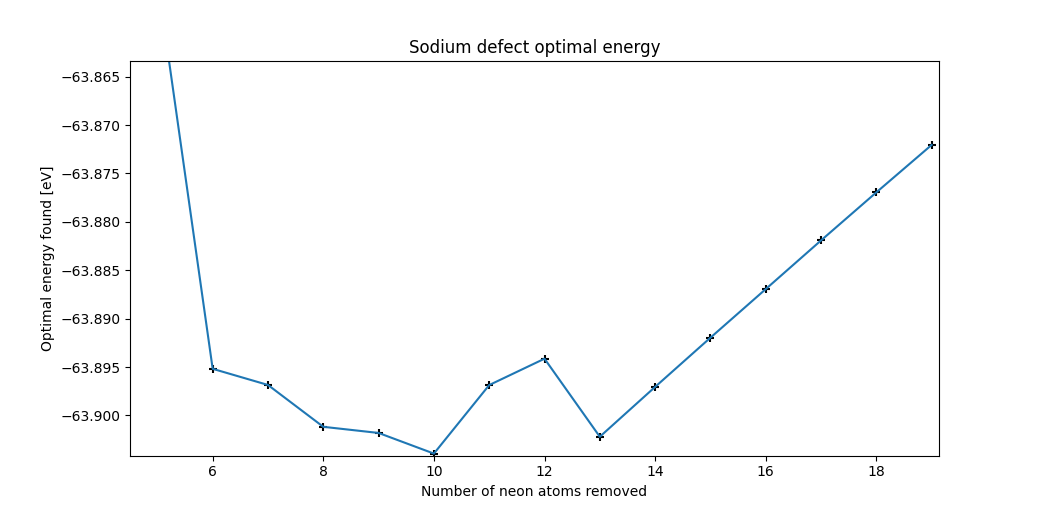
\includegraphics[scale=0.5]{./Inhalt/Bilder/optimal_defect_brute_force.png}
	\caption{Brute force for single sodium atom}
	\label{fig:bruteforcesodium}
\end{figure} 

\section{Sodium Dimer}
-maybe think about symmetry\\
-same graphics as for the monomer case\\
-heuristically take the maxima of these plots \\
-give structures\\
-discuss structures (inner shell carved out)\\

\chapter{DFT optical spectra results}
\label{chap:Zweites Kapitel}
%
Zweites Kapitel
%
%



\chapter{Erstes Kapitel}
%
%
\section{Einrichten dieser Vorlage}
\label{sec:Einrichten dieser Vorlage}
%
$\rightarrow$ Füge in der main.tex alle relevanten Metainformationen wie Titel, Autor, ... usw. ein.\\\\
%
$\rightarrow$ Ersetze das Logo in \textit{Inhalt/Bilder/logo.png} mit dem passenden Logo und passe ggf. den Dateinamen und -endung in \textit{Sonstiges/Titelblatt.tex} an\\\\
%
$\rightarrow$ Passe den Anhang in \textit{Verzeichnisse/Anhang.tex} entsprechend an.
%
%
\section{Drucken}
\label{sec:Drucken}
%
In der \textit{main.tex}:
\begin{itemize}
    \item oneside in twoside ändern
    \item openright einkommentieren
    \item  Den Befehl \textbackslash myemptypage hinter dem Titelblatt einkommentieren
\end{itemize}
%
In \textit{Config/Packages.tex}: 
\begin{itemize}
    \item alle farblichen links im hyperref package auskommentiern
\end{itemize}
%
In \textit{Config/Seitenstil.tex}: 
\begin{itemize}
    \item  pagemark von \textbackslash cfoot\{\} in \textbackslash ofoot\{\} tauschen
\end{itemize}
%
%
\section{Text}
\label{sec:Text}
%
Lorem ipsum dolor sit amet, consectetur adipiscing elit. Nullam placerat, dui ac vulputate commodo, est mi sagittis ipsum, sed ullamcorper nunc mauris eu sem. Vestibulum egestas, eros eu rhoncus suscipit, tortor diam molestie libero, in aliquam nisl lectus in dui. Quisque aliquet metus ut nisi volutpat, in hendrerit lectus porta. Etiam efficitur elit purus, vitae fringilla elit tempor ac. Aenean nec ipsum dictum, fringilla lectus a, aliquam neque. Nulla nec ante ut lectus sollicitudin elementum quis ac mi. Praesent a tellus magna.\\\\
%
Cras eget nulla dignissim, dictum libero non, consectetur elit. Nulla felis lorem, consequat sit amet interdum non, tincidunt eget leo. Integer mollis fringilla elit sit amet posuere. Fusce porttitor massa augue, ut faucibus risus lobortis at. Quisque lacinia erat in cursus sodales. \\
Donec aliquam lorem feugiat nibh dapibus, at blandit erat pretium. Aliquam erat volutpat. Quisque tempus dui at augue aliquet mattis. Aliquam erat volutpat.
%
%
\section{Bilder}
\label{sec:Bilder}
%
Bilder in dem Ordner \textit{Inhalt/Bilder} hinterlegen.
%
\begin{figure}[htpb]						
    \centering
    
\includegraphics[width=.3\textwidth]{Inhalt/Bilder/placeholder_image.png}
    \caption{Placeholder Image}
    \label{fig:placeholder} 
\end{figure}
%
%
\section{Programmcode}
\label{sec:Programmcode}
%
Programmcode in dem Ordner \textit{Inhalt/Code} hinterlegen.
%
\lstinputlisting[
    float=htpb,
    language=Python,
    label=lst:codeplaceholder,
    caption={Code Placeholder},]
    {Inhalt/Code/code_placeholder.txt}
%
%
\section{Tabellen}
\label{sec:Tabellen}
%
\href{https://www.latex-tables.com/}{Zum einfacheren erstellen von Tabellen}
%
\begin{table}[htpb]
    \centering
    \caption{Placeholder table}
    \label{tab:placeholder} 
    \begin{tabular}{ll}
    Spalte 1 & Spalte 2  \\ 
    \hline
    a        & 1         \\
    b        & 2         \\
    c        & 3        
    \end{tabular}
\end{table}
%
%
\section{Zitieren}
\label{sec:Zitieren}
%
Hier ein einfaches Zitat \cite{bibkey}.\\\\
%
Bibliographie Einträge in \textit{Verzeichnisse/Literatur.bib} hinterlegen.
%
%
\section{Abkürzung}
\label{sec:Abkürzung}
%
Abkürzungen in dem Ordner \textit{Verzeichnisse/Abkürzungsverzeichniss.tex} hintelegen.\\\\
%
Beim ersten Verwenden wird die Abkürzung ausgeschrieben, beim zweiten mal wird nur die Abkürzung benutzt.\\\\
%
Erste Verwendung: \ac{API}\\
Zweite Verwendeung: \ac{API}
%
%
\section{Aufzählungen}
\label{sec:Aufzählungen}
%
Normale Aufzählung:
%
\begin{itemize}
    \item Stichpunkt 1
    \item Stichpunkt 2
    \item Stichpunkt 3
\end{itemize}
%
Aufzählung mit custom Symbolen:
%
\begin{itemize}
    \item[xyz] Stichpunkt 1
    \item[abc] Stichpunkt 2
    \item[!] Stichpunkt 3
\end{itemize}
%
%
\section{Referenzieren}
\label{sec:Referenzieren}
%
Eine Referenz zu unserem Bild \ref{fig:placeholder}\\
Eine Referenz zu unserer Tabelle \ref{tab:placeholder}\\
Eine Referenz zu der Section Bilder \ref{sec:Bilder}
%
%
\section{Textstyle}
\label{sec:Textstyle}
%
\textit{Kursiver Text}\\
\textit{Bold Text}\\
\texttt{Mono Spaced Text} (Für bsp. Programmcode)
%
%
\section{Formeln}
\label{sec:Formeln}
%
\href{https://en.wikibooks.org/wiki/LaTeX/Mathematics}{Referenz für Mathematik in Latex}
%
\begin{align}
	\label{eq:input_gate}
	\Gamma_I &= \sigma\left(W_{I}\left[h_t|X_t\right]\right)&&\quad\text{(Input Gate)}\\
	\label{eq:output_gate}
	\Gamma_O &= \sigma\left(W_{O}\left[h_t|X_t\right]\right)&&\quad\text{(Output Gate)}\\
	\label{eq:forget_gate}
	\Gamma_F &= \sigma\left(W_{F}\left[h_t|X_t\right]\right)&&\quad\text{(Forget Gate)}
\end{align}
%
Symbolbeschreibungen werden in dem Symbolverzeichniss unter \textit{Verzeichnisse/Symbolverzeichniss.tex} hinterlegt.\\\\
%
So werden Formeln im Text angegeben $x^2$ und so kann man im Text einen übersichtlicheren Bruch verwenden $\nicefrac{kg\,m}{s^2}$.
%
%
\section{Sections}
\label{sec:sections}
%
\subsection{subsection}
\label{subsec:subsection}
%
\subsubsection{subsubsection}
\label{subsubsec:subsubsection}
%
%
